\subsection{\label{subsec:FZV2}Interferenz}
In Abbildung \ref{fig:refle} ist eine Skizze dargestellt, anhand der wir die 
konstruktive Interferenzbedingung anschaulich herleiten.
\begin{figure}[h!]
    \centering
    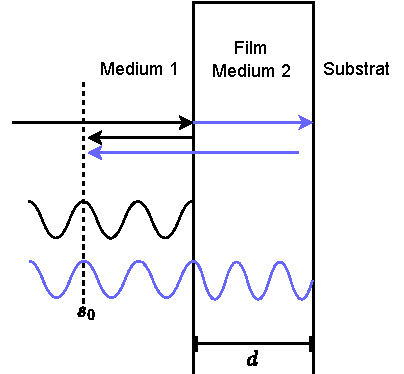
\includegraphics[width=0.5\textwidth]{Refle.pdf}
    \caption{\label{fig:refle}Skizzenhafte Darstellung einer ebenen Wellenfront, 
    die von Medium 1 auf einen Film auf einem Substrat trifft. Die Dicke des Films ist 
    durch $d$ gegeben. Die entstehenden Teilstrahlen überlagern sich wieder, wobei der 
    Punkt $s_{0}$ beliebig gewählt ist und als Berechnungsstütze fungiert. }
\end{figure}\FloatBarrier
Die einlaufende ebene Welle von der linken Seite (dargestellt in Schwarz) wird teilweise 
an der Grenzfläche des Films reflektiert. 
Der transmittierte Anteil (in Blau) wird wiederum an der Grenzfläche zum Substrat reflektiert. 
Dadurch entstehen zwei Teilstrahlen, die sich miteinander überlagern. 
Konstruktive Interferenz tritt auf, wenn sich die beiden ebenen Wellen so überlappen, 
dass beispielsweise die Wellenberge zweier Wellen an einem bestimmten Punkt $s_{0}$
aufeinander fallen. Wir berechnen die benötigte Zeit, damit die beiden Teilwellen den Punkt 
$s_{0}$ erreichen, wobei wir die unterschiedlichen Phasengeschwindigkeiten berücksichtigen. \newpage
Der Ursprung für diese Berechnung ist frei wählbar und wird an der Grenzfläche des 
Films zum Medium 1 gesetzt
\begin{align}
    t_{1} &= \frac{s_{0}}{v_{\text{ph,}1}} \\
    t_{2} &= \frac{s_{0}}{v_{\text{ph,}1}} + \frac{2d}{v_{\text{ph,}2}} \\
    \Rightarrow \Delta t &= \frac{2d}{v_{\text{ph,}2}} = \frac{2dn_{\text{Film}}}{c}.
\end{align}
Die zeitliche Differenz zwischen den Wellenbergen muss so gewählt werden, dass sich
wieder zwei Berge überlagern, was gegeben ist, wenn die in der Differenzzeit zurückgelegte 
Strecke einem ganzzahlig Vielfachem der Lichtwellenlänge entspricht. 
Es folgt
\begin{align}
    \Delta t &\stackrel{!}{=} \frac{m\lambda}{v_{\text{ph,}1}} = \frac{2dn_{\text{Film}}}{c} \\
    \Rightarrow \lambda &= \frac{2dn_{\text{Film}}}{m}, \,\,\,m\,\in\,\mathbb{N}\label{eq:inter}
\end{align} 
wobei zu beachten ist, dass die Wellenlänge $\lambda$ die Wellenlänge im Medium 1 repräsentiert, 
welche sich von der Vakuumwellenlänge je nach Brechungsindex des Mediums unterscheiden kann. \\
Zusätzlich muss beachtet werden, dass bei Reflexionen am optisch dichteren Medium Phasensprünge auftreten, 
die einen Gangunterschied von $\lambda / 2$ bewirken, dieser Gangunterschied ist am Übergang von 
Medium 1 zum Film und von diesem zum Substrat zu berücksichtigen und kann 
nachträglich zu Gl.~\eqref{eq:inter} ergänzt werden [Lehrbuch suchen + Skript]. \\